


%\chapter{The FACET E210 Experiment}
In 2014 the experimental campaign  for demonstrating the proof-of-concept of Trojan Horse injection (see \ref{sec:Theory_TrojanHorse}) started at the Facility for Advanced Accelerator Experimental Tests (FACET) at the SLAC national laboratory as the experiment E210. It was a collaborative effort with researchers from the University of Hamburg, University of California Los Angeles (UCLA), University of Strathclyde Glasgow and Radiabeam technology with a devoted support from the SLAC personnel. The FACET experiments had to be designed to be non-excluding, which led to a fruitful joint learning process between several groups.
It is fair to say that E210 was one of the most complex and accuracy-wise most demanding experiments conducted so far at FACET. 
Several steps were required in improving the overall setup, until the experiment was eventually successful.
The most crucial obstacles to overcome were timing and alignment between two laser arms and the electron beam.
The timing requirements between the electron beam and the pre-ionization laser are rather soft as long as the pre-ionization occurs before the arrival of the electron beam an with a timing difference less then the recombination time (ns-µs range). However, proper control over relative time-of-arrival between the injection laser and the electron beam required - in principal - control over timing on the order of $10\ \mathrm{fs}$. With an expected timing jitter in the range of $200\ \mathrm{fs}$ the best solution here was to accurately measure the relative TOA with an electro-optical sampling (described in\ref{sec:EOS}) to determine the injection properties from the data, rather than hope for live-control. 
For finding the synchronization ($t_0$) as well as fine-alignment between electron beam and injection laser, a newly observed effect on the plasma glow described in \ref{sec:Plasma_Glow} was measured and applied.

\section{The FACET experimental setup}
\subsection{LINAC}
\subsection{The FACET laser system}
Good description of FACET laser system in \cite{Green_FACET_Laser_PIOP}
\subsection{E210 setup}
\begin{figure}[htbp]
\includegraphics[width=0.9\textwidth]{experiment/images/raw/E210Setup.pdf}
\caption{}
\label{img:E210_Setup}
\end{figure}


\subsection{Imaging spectrometer}
The imaging spectrometer consists of a dipole and three 
\subsection{Laser energy calibration}
The FACET laser system ...
The energy that can be used on target of the OAP is controlled at two points in the laser-beamline.
At each point a cube-polarizer is surrounded by two  $\lambda/2$-waveplates, where the upstream one is motorized.
The main energy waveplate is located in the laser-room and the probe-energy waveplate is located in the tunnel area shortly after the split between main laser path and probe laser path at the main sampler, which means that the probe laser energy is determined by both waveplate settings while the main laser energy is set by the main laser energy waveplate only. From the power-meter in the laser-room, that measures shot-by-shot laser pulse energy, all the way down to the tunnel a variety of optical components are used until the laser is finally focused onto the 
The typical shot-to-shot laser energy jitter  is $\approx 5 \%$ FWHM.

Manta Cameras: \cite{GigE125_datasheet}

\begin{figure}[htbp]
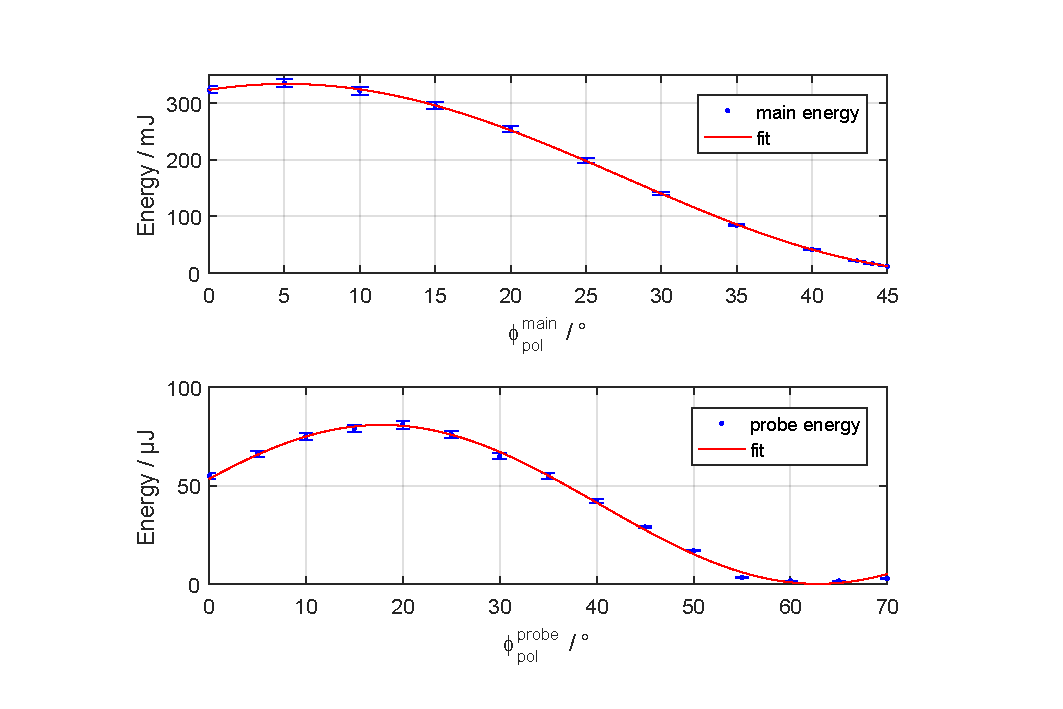
\includegraphics[width=0.9\textwidth]{experiment/images/edited/waveplate_calibration.pdf}
\caption{Laser energy calibration for main energy waveplate (upper plot) and probe energy waveplate (lower plot)}
\label{img:LaserEnergyCalib}
\end{figure}

All measured losses in optical components combined with the fitted functions for the waveplate energies (see figure \ref{img:LaserEnergyCalib}) combined give the on target energy applicable by axilens and OAP respecively.

\begin{align*}
 W_\mathrm{Laser}^\mathrm{OAP} &= W_\mathrm{Laser}^\mathrm{Laserroom}\times 1.25\times10^{-2}\\ 
 &\times\big( 0.994 \cos^2((\phi_{pol}^{main}-5.11\degree)) +6.16\times 10^{-3}\big)\\
  &\times \big(0.998 \cos^2((\phi_\mathrm{pol}^\mathrm{probe}-17.8\degree )) +1.65\times 10^{-3}\big)
\end{align*}

%\begin{align*}
% W_\mathrm{Laser}^\mathrm{OAP} &= W_\mathrm{Laser}^\mathrm{Laserroom}\times 1.25\times10^{-2}\\ 
% &\times\big( 0.994 \cos^2((\phi_{pol}^{main}-5.11\degree)) +1.16\times 10^{-3}\big)\\
%  &\times \big(0.998 \cos^2((\phi_\mathrm{pol}^\mathrm{probe}-17.8\degree )) +1.62\times 10^{-3}\big)
%\end{align*}

\begin{align}
 W_\mathrm{Laser}^\mathrm{Axilens} &= W_\mathrm{Laser}^\mathrm{Laserroom}\times 0.253\\
  &\times\big( 0.994 \cos^2((\phi_\mathrm{pol}^\mathrm{main}-5.11\degree)) +6.16\times 10^{-3}\big)\\
\end{align}

%\begin{align}
% W_\mathrm{Laser}^\mathrm{Axilens} &= W_\mathrm{Laser}^\mathrm{Laserroom}\times 0.253\\
%  &\times\big( 0.994 \cos^2((\phi_\mathrm{pol}^\mathrm{main}-5.11\degree)) +1.16\times 10^{-3}\big)\\
%\end{align}


This means that for a typical laser energy output of $500\, \mathrm{mJ}$ a maximum energy of $6.2\, \mathrm{mJ}$ on OAP target and $125.9\,\mathrm{mJ}$ on axilens could be used.
\subsubsection{Energy limitations}

\begin{equation}
E e^{-i(\omega t-kx)}=E e^{-i\omega(t-\frac{x}{c}(n_0+n_2 I) )}
\end{equation}

The maximum energy that can be applied for the OAP ionization is additionally limited by the damage threshold of the windows.  Three 
\begin{enumerate}
\item Intensity
\item The Fluence damage threshold for a 560 fs 248 nm laser pulse is measured \cite{mann1993damage} to be $1.70\ \frac{J}{cm^2}$. Measurements with a 55 fs 800 nm laser pulse in \cite{LiMgF2DamageThresh} indicate that the threshold is lower than $2\ \frac{J}{cm^2}$
\item Nonlinear effects: B<1
\end{enumerate}
\begin{equation}
B=\frac{2\pi}{\lambda}\int_0^{x}n_2(x')I(x')dx'
\end{equation}
The injection laser is coupled into the OAP chamber through a 
a 3 mm thick $\mathrm{MgF}_2$ window with an anti-reflection coating. By having the OAP in vacuum, more freedom of alignment is possible and focusing through a window is avoided, which could otherwise distort the laser focus or induce damage to the mirror.
$\mathrm{MgF}_2$ is the material of choice because of its low nonlinear refractive index value of  $n_2(\mathrm{MgF}_2)=0.763\times 10^{-16}\frac{cm^2}{W}$\cite{Nonlin_refr_index_PRB1989}.
The injection laser transverse profile can be approximated by a flat-top with a beam diameter of $10\ \mathrm{mm}$. 
Then the energy maximum for $B=1$ is $24.1\ \mathrm{mJ}$. That corresponds to a Fluence of $30.6 \frac{\mathrm{mJ}}{\mathrm{cm}^2}$ and an intensity of $5.6\times 10^{11}\frac{\mathrm{W}}{\mathrm{cm}^2}$


\section*{Timing jitter estimate}
In order to establish a controlled injection of electrons into the wake, a synchronisation between electron beam and laser pulse on the order of few 10th of fs is desirable. 
The Vitara-T laser main oscillator is mode-locked to the master reference of the radio-frequency (RF) master reference \cite{Green_FACET_Laser_PIOP}. This lock according to \cite{Green_FACET_Laser_PIOP} has a timing jitter of 
\begin{equation}
\sigma_{t}^\mathrm{RF,laser}=70\ \mathrm{fs}.
\end{equation}

The electron bunch on the other hand has a timing jitter with respect to the RF, which
can be estimated with linear beam-optics as described in equation \ref{eqn:R_Matrix}.
Due to energy-dependent path lengths in the W-chicane the electron beam energy jitter translates into a  timing offset with the relation
\begin{align}
\sigma_{t}^\mathrm{e^-,RF}&\approx \Delta z_\mathrm{f}/c \\
&=R_{56}\delta_\mathrm{i}/c.
\end{align}
The sector 20 chicane $R_{56}$ is typically set to $-7\ \mathrm{mm}$ to achieve maximum bunch compression  and the rms energy jitter 
has been measured to be $\delta_\mathrm{i}= \frac{18.7\ \mathrm{MeV}}{20.35\ \mathrm{GeV}}=9.2\times10^{-4} $\cite{ThesisGessner} so that the rms time of arrival jitter of the electron beam with respect to the master RF reference can be estimated to be 
\begin{equation}
\sigma_{t}^\mathrm{e^-,RF}\approx\ 21.5\ \mathrm{fs}.
\end{equation} 
Additional laser time-of-arrival jitter due to pointing jitter is small enough that its' contribution can be ignored.
This leaves us with a total estimated laser pulse to electron time-of-arrival jitter of

\begin{equation}
\sigma_{t}^\mathrm{e^-,laser}=\sqrt{(\sigma_{t}^\mathrm{e^-,RF})^2+(\sigma_{t}^\mathrm{RF,laser})^2}=73.2\ \mathrm{fs}.
\end{equation}
Keeping in mind that this is a rather optimistic estimate and long-term drifts might need adjustment to find the right timing such a jitter value requires a direct measurement of the 
relative TOA.

\section{Electro Optical Sampling (EOS)}
\label{sec:EOS}


Electro-optical sampling is a method that is perrfectly suited for determining such time-differences in Time-of-arrival between a laser-pulse and a Thz-source, as e.g. an ultra relativistic electron-beam, by exploiting the properties of optically anisotropic crystals and has been shown to be able to measure sub-picosecond electron bunches \cite{YanX_EOS_PRL2000}.

Electromagnetic waves, propagating through anisotropic crystals perceive a difference in dielectric permitivity $\epsilon_\mathrm{r}$, depending on entrance angle and polarization of the wave, which is why in a more general way the dielectric properties need to be addresses with the dielectric permitivity tensor  $\hat{\epsilon}$.
This is equivalent to a polarization-depending index of refraction, a property known as birefringence, which leads to a polarization-dependent phase velocity of light inside the crystal. 
A laser at the correct incident angle with respect to an anisotropic crystal will therefore notice a phase shift between different planes of polarization which leads to an overall change in the laser polarization, depending on the phase shift strength and the crystal size. 
Electro-optical crystals change the orientation of the dielectric permitivity tensor when an external electric field $\vec{E}_\mathrm{ext.}$ is applied.
The strength of this effect can be illustrated by taylor-expanding the impermeability tensor 


\begin{equation}
\hat{\eta}=\hat{\epsilon}^{-1}
\end{equation}
for small external electric fields $\vec{E}_\mathrm{ext.}$ to
\begin{equation}
\eta_{ij}=\eta_{ij}(0)+r_{ijk}E_k+s_{ijkl}E_k E_l+...\ .
\end{equation}
The linear dependency on the electric field strength is called Kerr-effect with $r_{ijk}$ being the Kerr-coefficient. 
The Pockels effect with the Pockels coefficient $s_{ijkl}$ describes quadratic dependency.
In the context of this work and the described experiment only two elctro-optical crystals were used, GaP and ZnTe. 
As both of them are packed in a zincblende geometry, which does not obtain an inversion center, the electro-optic effect is dominated by the Pockels-effect.

\subsection*{EOS setup}
In order to measure the relative time-of-arrival between electron bunch and laser pulse an Electro optical sampling (EOS) was set up as a non-destructive shot-by-shot diagnostic.

In this experiment the crystal is located in close proximity (few mm distance) to the electron beam axis. Due to the high $\gamma_\mathrm{b} \approx 42000$ , the beam electric field is strongly lorenz-contracted and can be assumed to temporally only extend for the length of the electron beam. Consequently the electric field applied to the crystal and with that the induced birefringence are only active while the electron beam passes by the crystal.  
Figure \ref{img:EOS_Setup} depicts the setup.
A linear polarized laser pulse (red), a pickup of the probe beam, traverses the crystal with an angle of $~ 45\degree$ with respect to the electron beam axis (green). The laser beam is collimated with a transverse diameter of $~ 1 cm $ and completely illuminates the crystal. For a better signal-to-noise ratio, an additional polarizing filter was installed prior to the picnic basket chamber. After the chamber follows a cross-polarized filter, which can remotely be rotated for alignment purposes.

During the measurement only the polarization of that transverse part of the laser which propagates through the crystal at the very moment in which the electron beam' electric field induces the birefringence will be rotated and not be filtered by the polarizing filter further  downstream the laser beam path. As a result the signal has the form of a line as seen in figure \ref{img:EOS_Signal} with a horizontal position linearly corresponding to the relative TOA.

\begin{figure}[htbp]
\center
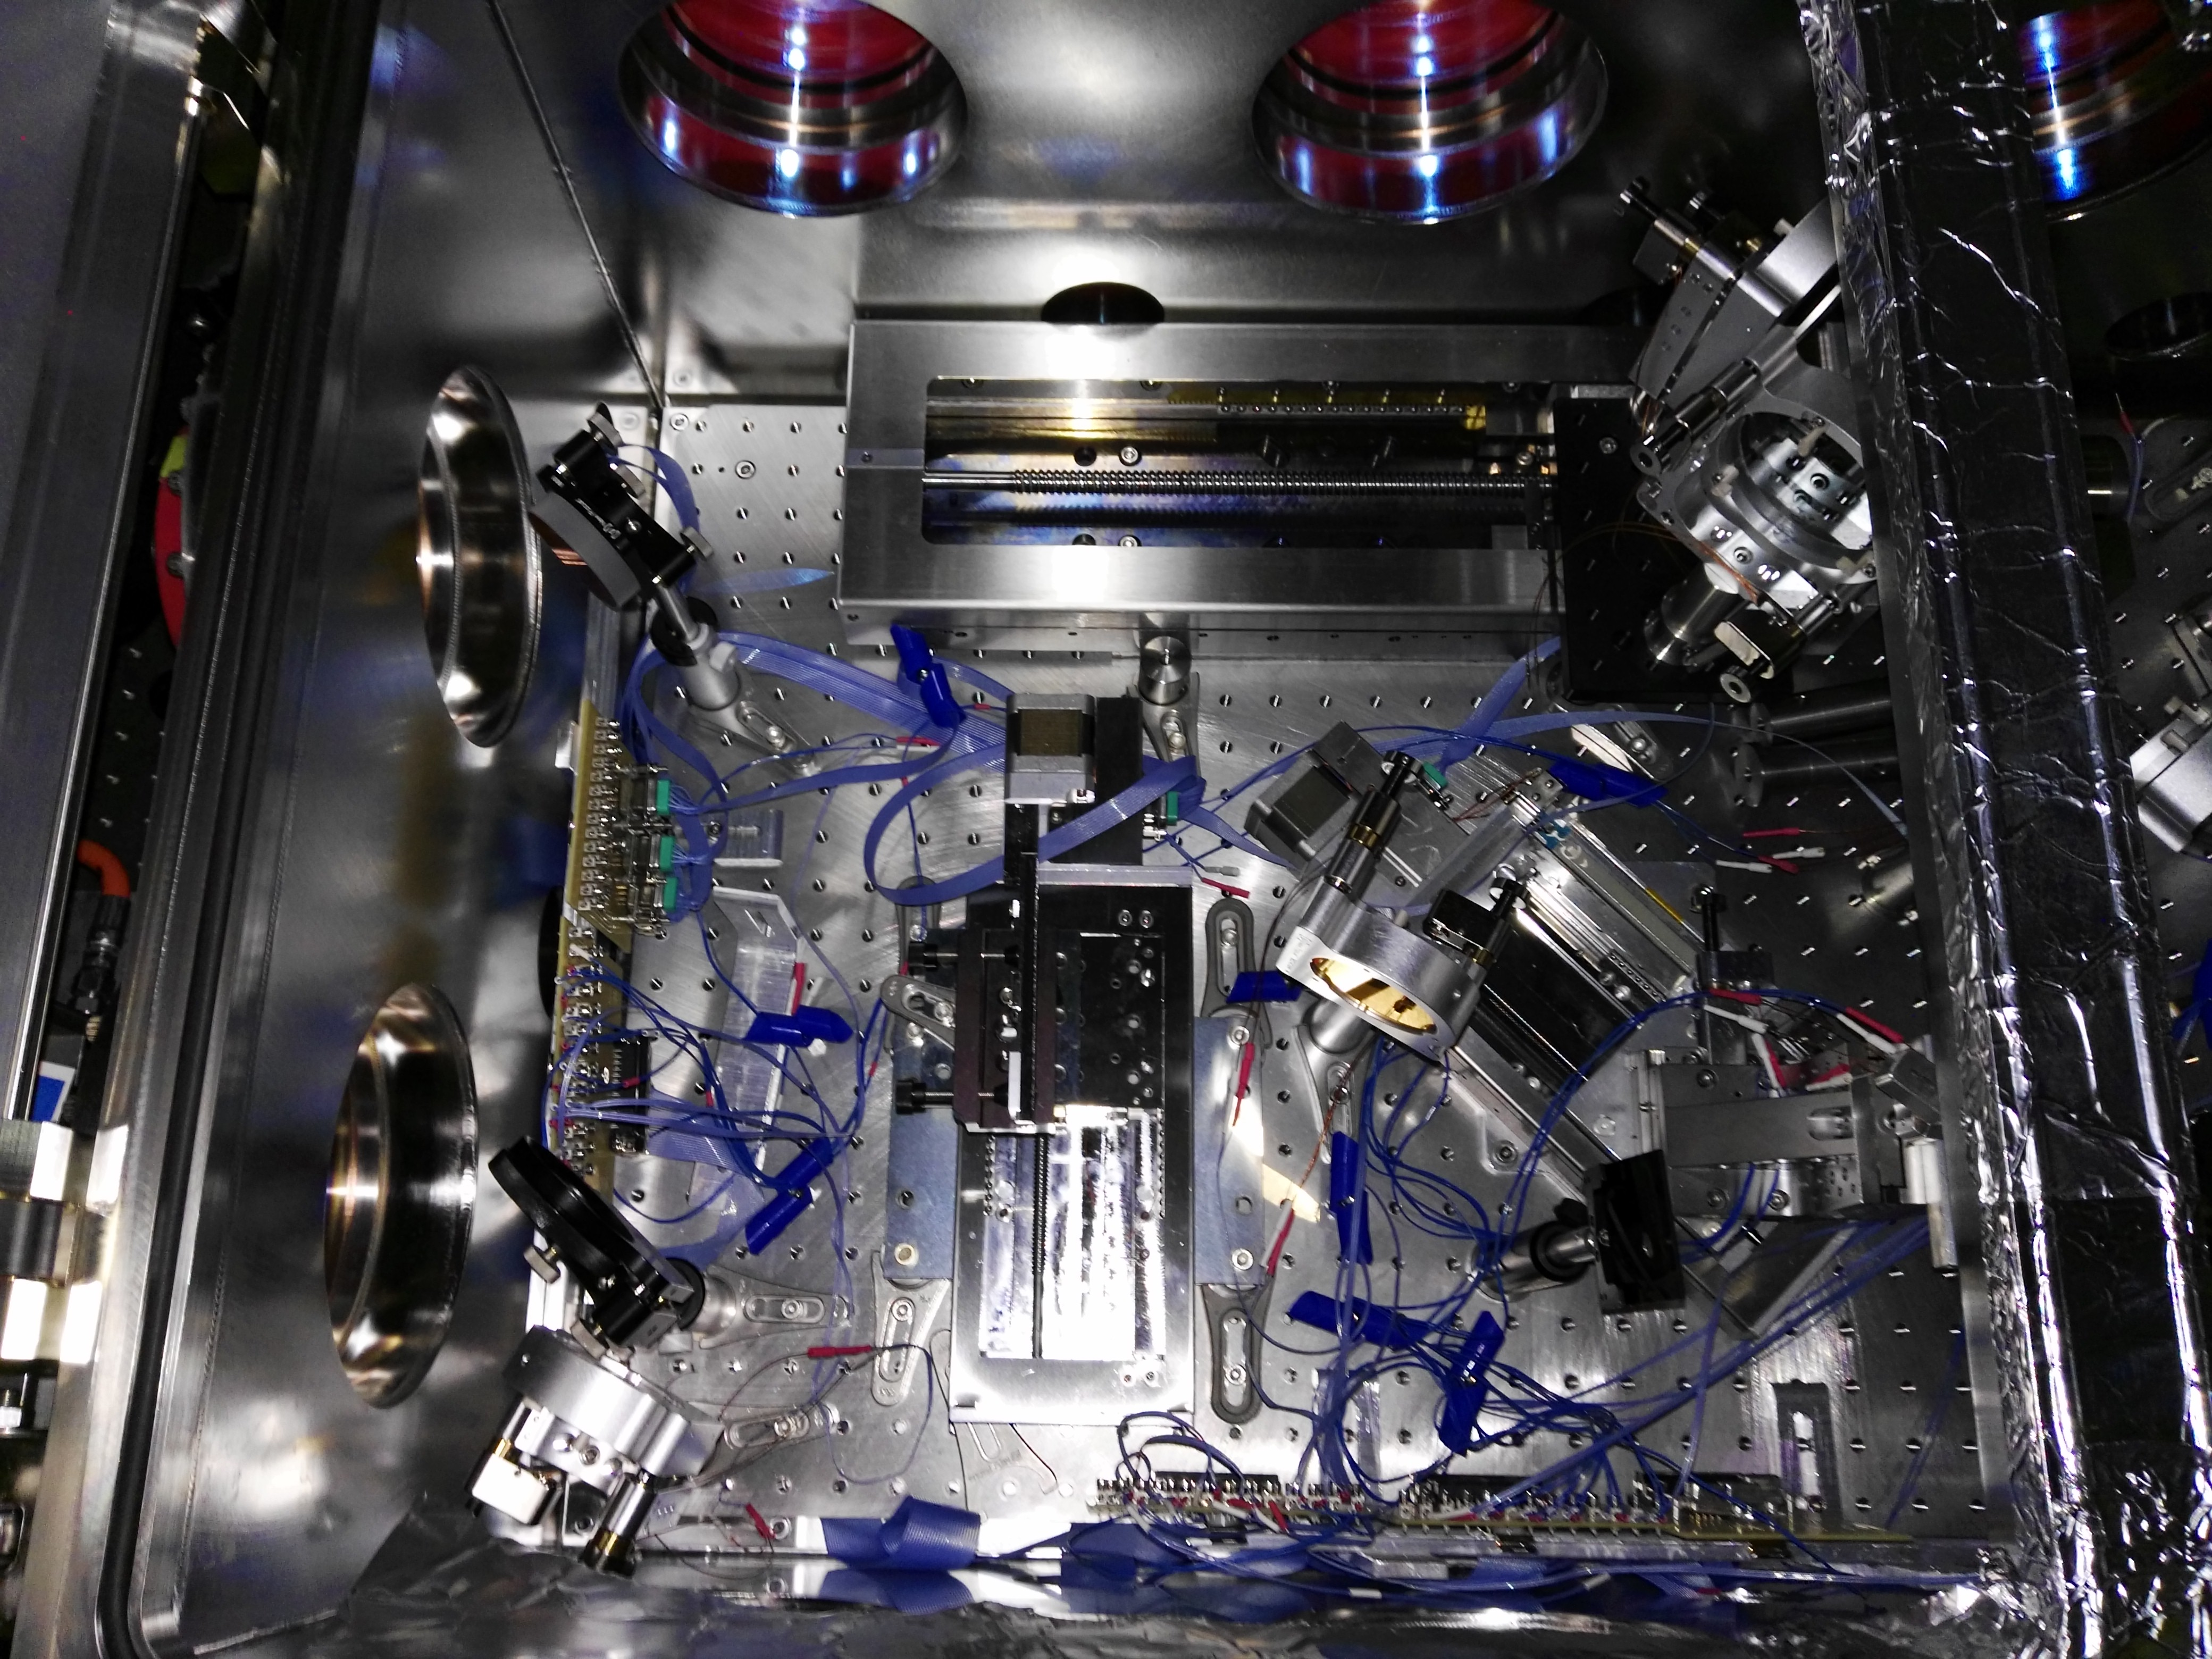
\includegraphics[width=1.0\textwidth]{experiment/images/edited/EOS_setup.pdf}
\caption{Setup of upstream electro-optical sampling inside the picnic basket chamber. Electron beam (green) and EOS laser (red) co-propagate in a small angle }
\label{img:EOS_Setup}
\end{figure}

The crystal plate is oriented perpendicular to the electron beam axis to minimize temporal overlap and the laser has an $\approx 40°$ angle with the electron beam which enables a correlation between signal position i.e. the part of the laser with rotated polarization and relative timing.

The entire ladder supports a YAG crystal to find the electron beam axis, a $500\ \mathrm{µm}$ thick ZnTe for broad timing scans and GaP with $100\ \mu\mathrm{m}$ thickness for fine resolution.
A detailed description of the physics involved in the application of electro-optical crystals as TOA and bunch length diagnostic can be found in \cite{BerndSteffenPhD}.


\begin{figure}[htbp]
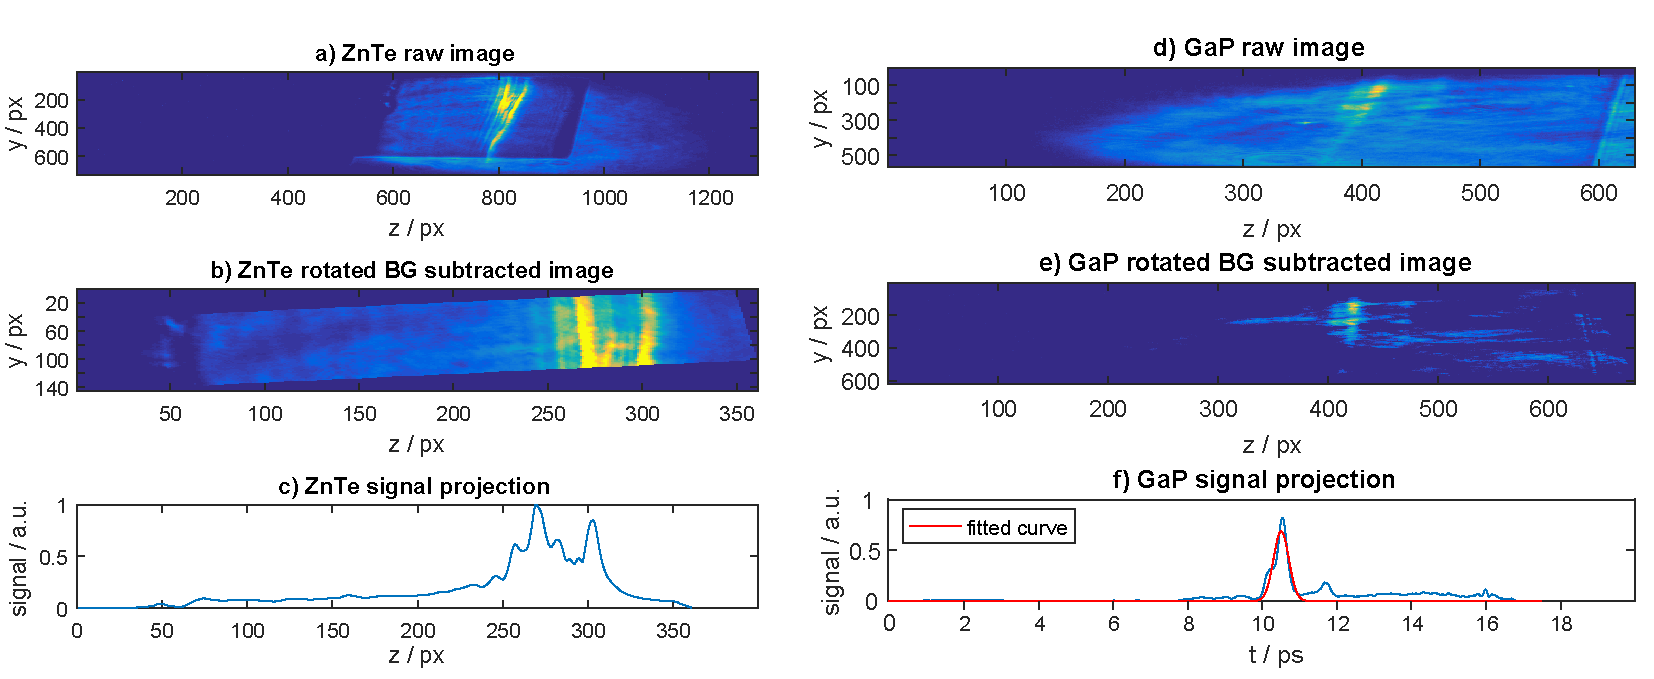
\includegraphics[width=1.0\textwidth]{experiment/images/edited/EOS_Signal.pdf}
\caption{EOS signal}
\label{img:EOS_Signal}
\end{figure}
\subsection*{EOS calibration}
The EOS signal can be seen in figure (\ref{img:EOS_Signal}). A small region of interest of the raw images (a,d) is rotated and the background, which mostly consists of the laser profile is  subtracted (b,e). The image projection shows a strong, but broad signal for the thick ZnTe crystal (c). The GaP signal is much cleaner. The Maximum position as well as a Gaussian fit is calculated to determine the relative timing.The EOS calibration was performed by changing the laser target time with respect to the RF main reference. For every time step several shots are performed to even out the timing jitter. We assume here that there is a timing jitter that behaves equally for every step in the data acquisition so that for a sufficient number of shots per time step the calibration becomes accurate. Taking too large datasets takes more time that drifts start to play a role. Therefore calibration result may vary from dataset to dataset. Furthermore calibration may vary from day to day due to deviation in laser alignment.
\begin{figure}[htbp]
\center
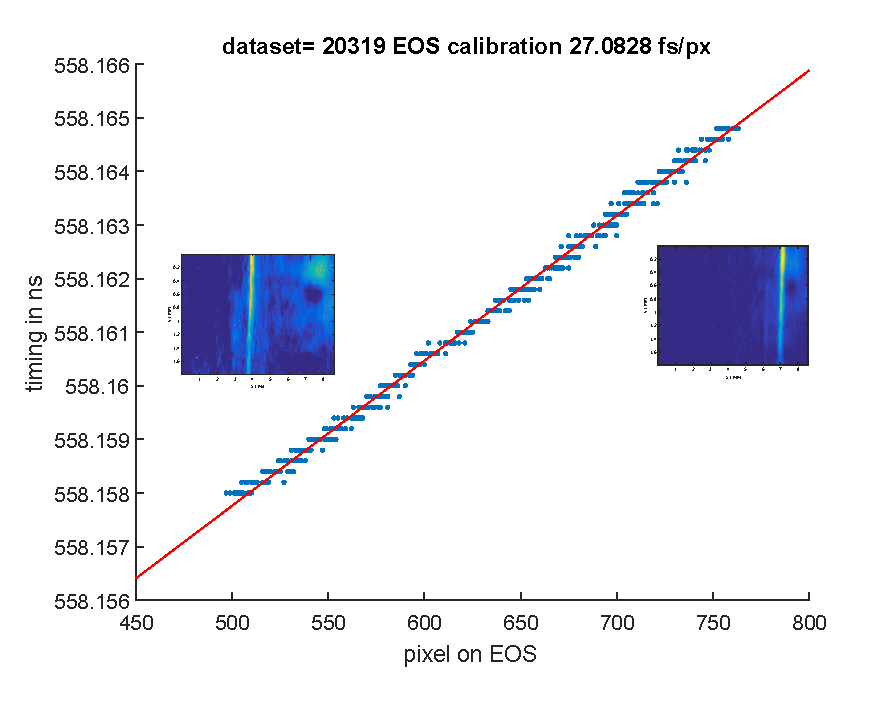
\includegraphics[width=0.5\textwidth]{experiment/images/edited/20319_EOS_calibration.pdf}
\caption{Typical EOS calibration}
\label{img:EOS_Calib}
\end{figure}

An EOS calibration is shown in figure (\ref{img:EOS_Calib}) with a clear linearity between signal position an timing as well as a slim scattering of the datapoints around the mean step value.
In principal such a calibration is not required with this method prior to performing timing scans for the sake of the actual experiment. As long as sufficient datapoints are taken per step a calibration can be obtained specific for any such dataset, which led to a multitude of calibration data. Taking into account several timing scans over several days we can conclude a mean calibration with confidence intervall
\begin{equation}
t_\mathrm{EOS}^\mathrm{calib}= 25.8\pm 2.5\ \frac{\mathrm{fs}}{\mathrm{px}} .
\end{equation}




\subsection*{Measurement of the TOA timing jitter}
With the calibrated EOS diagnostic one can now determine the actual relative timing jitter between electron beam and laser pulse and compare it with our estimate. Taking 1000 consecutive shots gives a measured timing jitter of  
\begin{equation}
\sigma_t^\mathrm{TOA} = 150.61\pm14.59\ \mathrm{fs}.
\end{equation}
This result shows that the previous estimate was indeed much too optimistic and that implementing the EOS diagnostic is a crucial tool to determine the shot-by-shot relative timing. One might now think about using this diagnostic now to pin down precisely the most predominant contributor to the timing jitter, which would have been a viable endeavor and could help in terms of stability. Thanks to the possibility to measure the timing shot-by-shot and non-invasive there was no need for this. The EOS gives us the freedom to operate and measure independent of the complex combination of short-term jitters long-term drifts, klystron malfunctions and the electron beam operation , which constantly requires small manual adjustments in order to maintain electron beam compression and alignment.

Moreover it gives is the possibility to sort our data by timing and investigate the physics depending on relative timing on a timescale of $\approx 30\ \mathrm{fs}$.
This sorting of data does not necessarily require an established calibration or any understanding about the current situation of the LINAC, as long as there is beam. The mere relative position of the EOS signal between different data points is sufficient for a sorting by time-of-arrival.

%\section{Torch kick}
%\begin{figure}[htbp]
%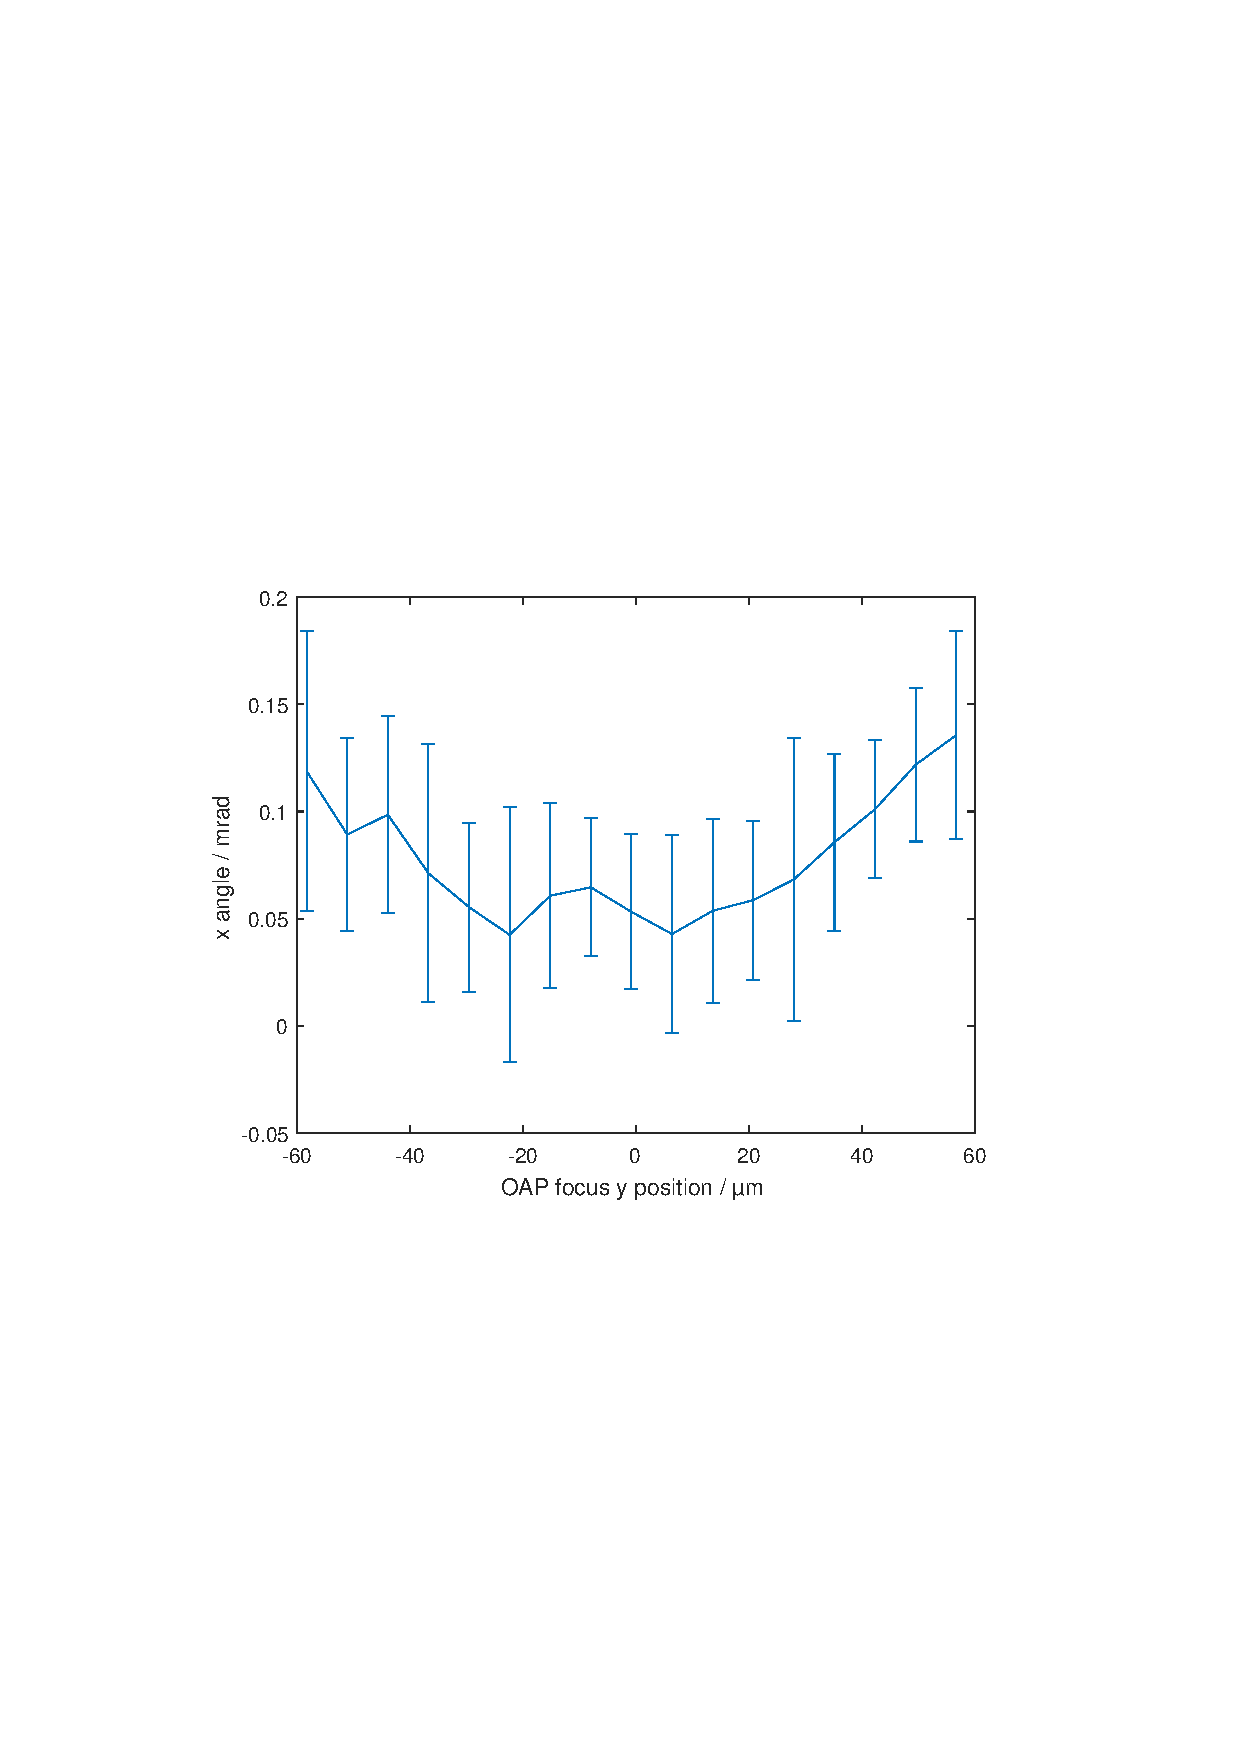
\includegraphics[width=0.9\textwidth]{experiment/images/raw/Torch_rollscan.pdf}
%\caption{'test'}
%\label{img:TochKick}
%\end{figure}


\section{Ionization test}


\section{Plasma glow diagnostic}
\label{sec:Plasma_Glow}
Section (\ref{sec:EOS}) describes the EOS commissioning and demonstrates that it is excellently suited for relative time-of-arrival measurements of electron beam an laser pulse. However, there is one detail, the EOS as it is set up is not capable of answering, which is  at which timing or range of timing electron beam and injection laser pulse do spatially overlap, so that they are in synchronization. 
Luckily it was observed before at FACET that the plasma light emission increased significantly if it was not only ionized by the laser, but also afterwards hit by the electron beam. 

Because this could be a potential solution to the synchronization problem we planned and performed a preparatory experiment to determine the time scales and physics of this transition. 
One huge advantage of the hydrogen FACET setup compared to the oven setup was that now several view ports allowed for observing the interaction. We set up a camera, observing cube 3 from bottom up and attached two band-pass filters on remote controllable flippers to it, one for  656$\pm$10 nm and one filter for ... nm.
The camera takes an integrates image over several $\mu$s, a time window, much larger than the plasma recombination time. The EOS then allows for sorting these images by TOA and measuring precisely the time scales.



\begin{figure}[htbp]
\center
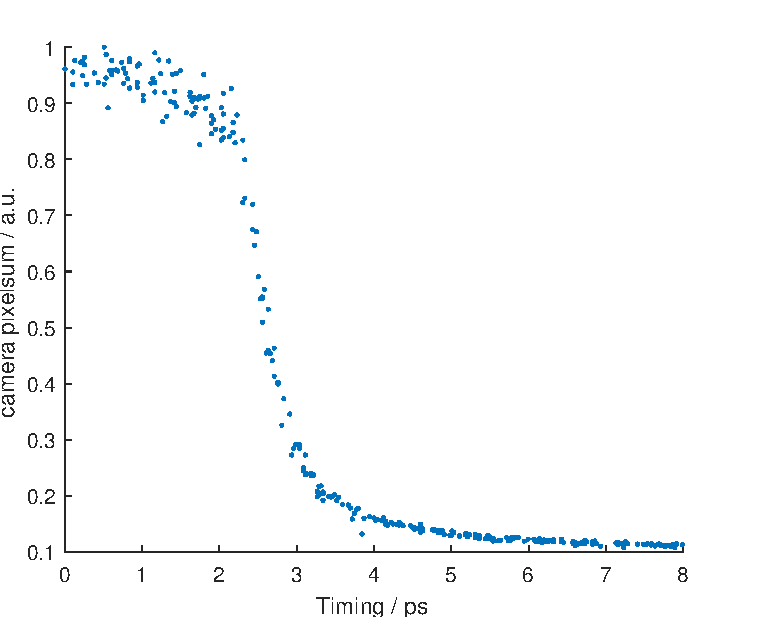
\includegraphics[width=1\textwidth]{experiment/images/raw/PlasmaGlow_20384_scatter.pdf}
\caption{Relative electron beam to injection laser timing scan. The pixel counts measured by the cube 3 vertical camera with a 656$\pm$10 nm  band-pass filter are sorted by the EOS. evaluation.}
\label{img:PlasmaGlowTimingOAP_H2He}
\end{figure}

Figure \ref{img:PlasmaGlowTimingOAP_H2He} shows the plasma glow accumulated intensity at the wavelength 656$\pm$10 nm , sorted by relative time-of-arrival between electron beam as measured by the EOS. The transition between a situation where the injection laser arrives earlier than the electron beam and vice versa is around $1\ \mathrm{ps}$ wide, which sufficiently fulfills the requirements to find a range of synchronization as the total range of the EOS crystal is around 20 ps ???.
During the data acquisition the electron beam charge was $3.1\pm \ 0.17\ \mathrm{nC}$. 

\begin{figure}[htbp]
\center
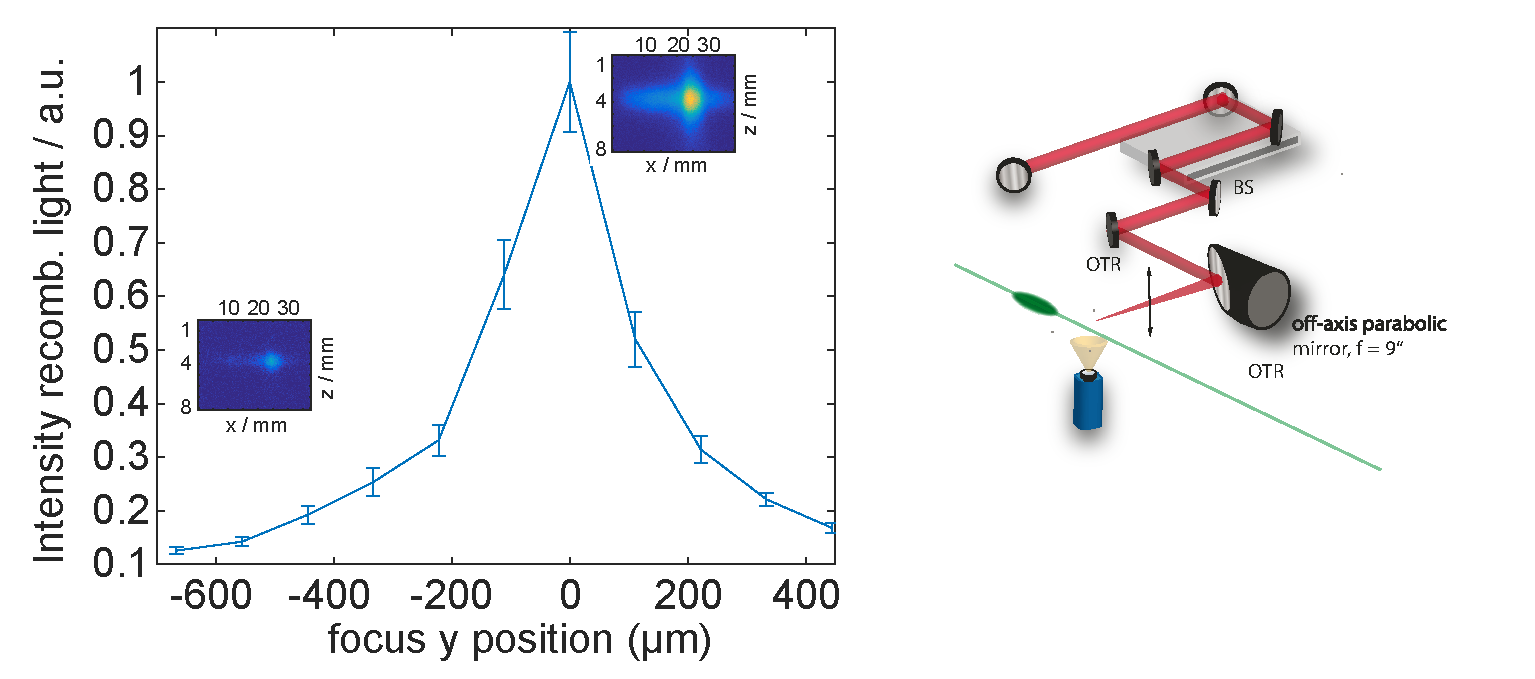
\includegraphics[width=1.0\textwidth]{experiment/images/edited/Plasma_Glow_roll.pdf}
\caption{Plasma glow in 7.8 torr $\mathrm{H}_2$ ( $n_\mathrm{e}=5\times10^{17}\mathrm{cm}^{-3} $) measured by vertical camera in cube 3. The injection laser off-axis parabola roll is scanned. The vertical plasma position is evaluated by the focus diagnostic.}
\label{img:PlasmaGlowRoll}
\end{figure}

\section{Charge calibration}
The witness beam charge is measured with two different methods, by comparing the total charge before and after the plasma section and from the intensity of a scintillating screen at the spectrometer.\\
Toroidal Current Monitors (toroids) before and after the plasma section seem to be the obvious diagnostic tool for additional charge. 
There are two reasons, however, why in this thesis the charge difference measured by the beam position monitors(BPMs) will be used instead. 
The first reason is that the toroids after the plasma section seemed to be vastly over-estimating the additional charge. Acceleration of several nanocoulomb in the plasma wake as sometimes given out by the toroids is, although maybe not impossible, hard to believe, especially when the BPMs show much more believable values. The thinking here is, that 
a direct hit of the toroid's conducting elements by spread out electrons after the plasma section might prompt to big of an response, while the BPMs from experience seem not to be prone to such a systematic error. 
\begin{figure}[htbp]
\center
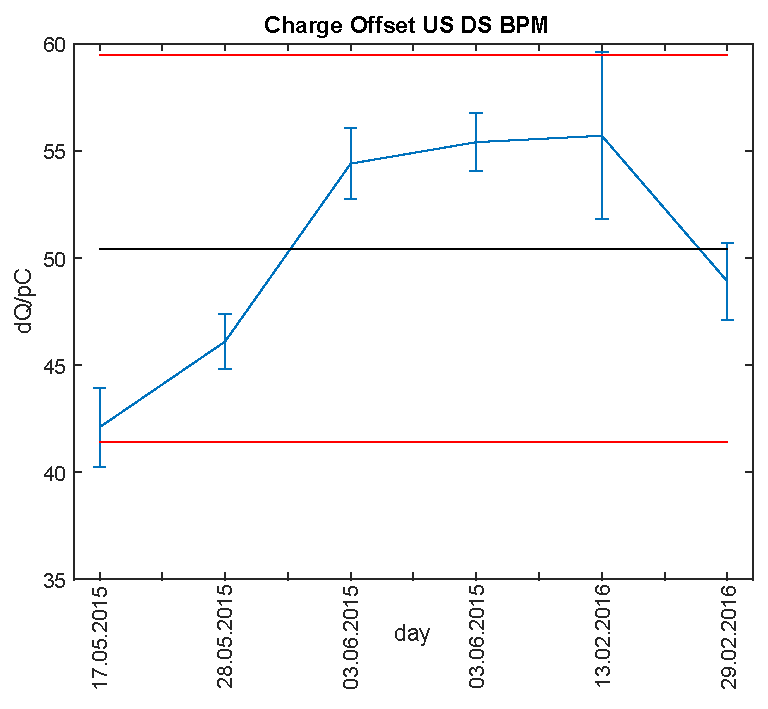
\includegraphics[width=0.5\textwidth]{experiment/images/edited/Charge_Tara.pdf}
\caption{s}
\label{img:Q_offset}
\end{figure}
The second reason is a more scientific one. 
In order to compare the charge before and after the interaction the measuring devices should balance to $\Delta Q =0$ in vacuum, or show a constant offset. Figure (\ref{img:Q_offset}) shows the offset between the charge measured by the  BPM nearest to the interaction point upstream (USBPM) and downstream (DSBPM) of it. Each datapoint shows the mean and the standard deviation of the shot-by-shot offset of a dataset. The black line depicts the long term mean of 
\begin{equation}
\Delta Q^\mathrm{offset}=50.4\pm 9.0\ \mathrm{pC}
\end{equation}
 with the long-term confidence-interval depicted by the red lines. Among all possible combinations of charge measuring devices the combination USBM and DSBPM showed the most stable long-term offset and variation per dataset.


\newpage

\begin{figure}[htbp]
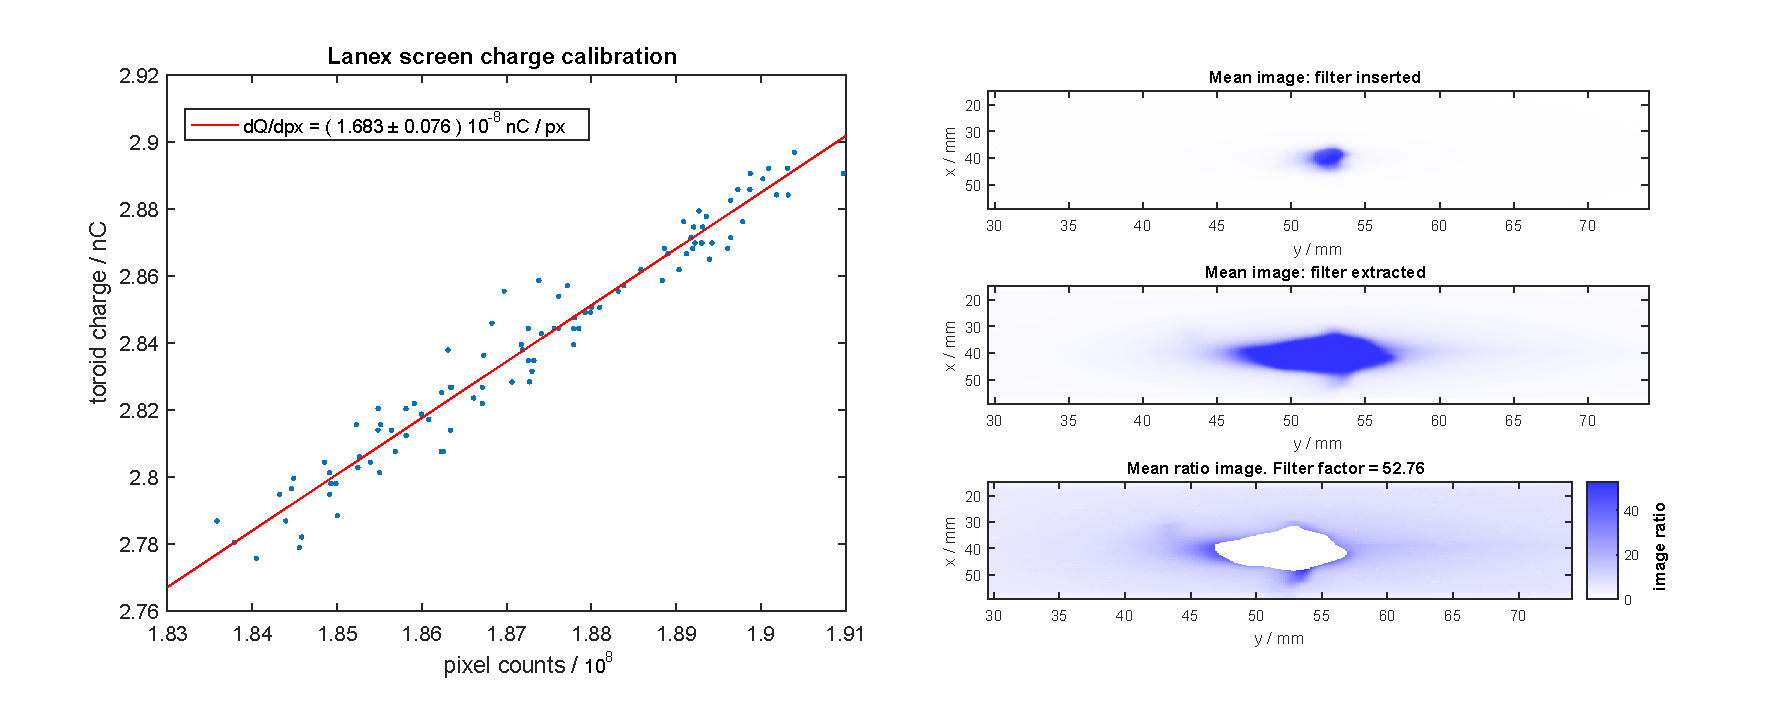
\includegraphics[width=1.0\textwidth]{experiment/images/edited/DRZ_charge_calib.pdf}
\caption{DRZ charge calibration}
\label{img:DRZ_ChargeCalib}
\end{figure}


Scintillating screens with a layer of phosphor - they go by by their brand name LANEX - are a successfully applied standard diagnostic for electron beams for several years now.
LANEX screens are an advantageous material because of their good radiation hardness and 
their linear scintillation response to charge over a large range of electron energies and charge densities \cite{buck2010LANEX}. While in Laser-driven accelerators a LANEX screen charge calibration can be a tedious task, in PWFA experiments a well understood electron beam is conveniently available. Figure (\ref{img:DRZ_ChargeCalib}) shows the analysis of the charge calibration. The full charge 3 nC FACET electron beam was scattered at a thin foil to avoid saturation of the screen. The image, after background subtraction was cleaned of additional signal from x-rays with a morphological opening filter. The calibration images were taken with an neutral density (ND) 2 (T=1/100) filter, but the witness beam data  is taken without this filter to guarantee detection of all witness beams. 
Therefore additionally images with, and without filter inserted were taken and compared. 
The most intense part of the filter-in image should be compared with the mean non-saturated filter-out image which gives a total filter factor of 52.76 and a calibration of 
\begin{equation}
Q_\mathrm{calib}^{DRZ}=88.795\pm 4.0 \times 10^{-5} \mathrm{pC/px}
\end{equation}





\subsection*{Result:}
With the 
\section{Result: Plasma Torch injection}
\section{Result: Trojan Horse injection}